\documentclass[11pt]{article}
\usepackage[final]{acl}
\usepackage{times}
\usepackage{latexsym}
\usepackage[T1]{fontenc}
\usepackage[utf8]{inputenc}
\usepackage{microtype}
\usepackage{inconsolata}
\usepackage{graphicx}
\usepackage{booktabs}
\usepackage{multirow}
\usepackage{subcaption}
\usepackage{amsmath}
\usepackage{url}

\setlength\titlebox{5.6cm}

\title{ManoVarta: Multilingual Conversational Screening for Mental Health}

\author{
  Ritwij \\
  Multilingual Mental Health Screening Project \\
  \texttt{ritwij@gmail.com}
  \And
  Yash \\
  Multilingual Mental Health Screening Project \\
  \texttt{team-collaboration}
}

\begin{document}
\maketitle

\begin{abstract}
ManoVarta is a multilingual, voice-capable screening system that converts open-ended English, Hindi, and Hinglish conversations into PHQ-9 and GAD-7 item-level evidence, scores, and safety decisions. The project did not succeed through raw prompting alone. Early direct-scoring and heuristic systems either abstained heavily or produced conversationally plausible but clinically thin outputs. The turning point was an evidence-first architecture: extract candidate symptom evidence, score only supported questionnaire items, and route safety through a separate hybrid stack. The final live runtime reaches \textbf{0.783} coverage completeness, \textbf{0.639} exact match, \textbf{0.251} macro-F1, \textbf{1.0/1.0} safety precision/recall, \textbf{0} parse failures, and \textbf{2.29} average user turns to a stable item score. We also document the actual model-selection path. A saved local Qwen probe and a later retrospective local Llama 3.1 8B probe were both informative, but Aya remained the best extractor choice because it was the first model family to deliver a strong archived multilingual evaluation rather than a narrow probe success. The final system therefore combines Aya-shaped extraction logic, hybrid safety, backend speech, and self-hosted local deployment.
\end{abstract}

\section{Introduction}
Validated instruments such as PHQ-9 and GAD-7 remain central to mental-health screening because they are interpretable, clinically familiar, and easy to score \citep{kroenke2001phq9,spitzer2006gad7}. Their rigid administration, however, often feels like a test rather than a conversation. ManoVarta targets this gap: instead of asking every item in order, it treats screening as a guided multilingual dialogue that still has to end in item-level evidence, confidence estimates, and an explicit safety state.

The most important lesson from the project is that conversational screening is not solved by asking a model to ``infer everything'' from raw dialogue. Our early runs showed the opposite: direct prompting could sound fluent while failing to cover the questionnaire in a usable way. Progress came from adding structure one layer at a time: evidence extraction before scoring, safety outside the main generator, confidence-aware follow-up planning, language-sensitive lexicons, and a verifier path for ambiguous English anxiety items. This report therefore concentrates on the measured path from weak baseline to live deployment rather than on planning-stage ideas that were never validated.

Three contributions matter most. First, we build a multilingual screening runtime grounded in PHQ-9 and GAD-7, with English and Hindi as the required languages and Hinglish treated as a realistic robustness condition. Second, we show that safety and coverage pull in different directions: the strongest offline extractor was not the best deployed system. Third, we document the actual model-selection trail, including saved Qwen evidence, Aya extractor results, DAIC-assisted continuation, hybrid safety fusion, and a final self-hosted runtime.

\section{Task, Data, and Evaluation}
The target output is an item-level screening summary: PHQ-9 and GAD-7 item scores in the 0--3 range, supporting evidence snippets, unresolved items, and a safety label (\texttt{none}, \texttt{review}, or \texttt{urgent}). We explicitly treat the system as a screening aid rather than a diagnostic or therapeutic agent \citep{abd2020chatbots,dosovitsky2021chatbot}. Safety is evaluated separately because crisis detection failure is qualitatively different from ordinary item-scoring error \citep{zirikly2019clpsych,pichowicz2025suicidal}.

The current data pipeline has two layers. \textbf{(A) Gold compliance pack:} 60 real audio+transcript sessions (30 English, 30 Hindi), each with profile metadata and a dual-annotation stack: \texttt{annotator\_a}, \texttt{annotator\_b}, and \texttt{adjudicated} files (180 label files total). The English side is sourced from E-DAIC public interview material, and Hindi from IndicVoices conversational recordings. The adjudication report over all 60 sessions shows 0.927 exact agreement and Cohen's $\kappa=0.7319$. \textbf{(B) Model-development exports:} processed multilingual screening data used by the extractor/follow-up/safety trainers, including 84/48/48 extractor train/dev/test examples, a 140-example \texttt{extractor\_train\_best} split, 126/80/84 safety train/dev/test items, and 120/96/144 follow-up train/dev/test instances. We also added DAIC-WOZ export support as an \emph{auxiliary English-only} supervision source, but did not treat it as the multilingual benchmark because DAIC-style prompts can bias models toward interviewer artifacts \citep{burdisso2024daic}.

\paragraph{Annotation governance.}
All 60 gold sessions were independently scored by two human annotators (A/B) using PHQ-9 and GAD-7 item anchors (0--3) with evidence-backed labeling. Disagreements were routed to an adjudication pass that produced one final adjudicated label file per session. Review work was tracked through reviewer queues and closed only when all three files (\texttt{annotator\_a}, \texttt{annotator\_b}, \texttt{adjudicated}) were present and schema-valid. This governance flow is what the strict compliance reports use for final claims; earlier AI-assisted bootstrap artifacts are treated as intermediate and not used for strict gold-label assertions.

We report four families of metrics. \textbf{Discourse effectiveness} uses coverage completeness, exact match, macro-F1, and parse failures. \textbf{Safety accuracy} uses precision and recall on live runtime endpoint evaluation. \textbf{Disclosure efficiency} measures how many user turns are required before an item score stabilizes and stays fixed. \textbf{Latency} is reported from the final assignment bundle as local screening-path latency; importantly, it excludes networked hosted-model round trips and therefore should be interpreted as core screening latency rather than full conversational UI delay.

\section{System Evolution}
\begin{figure*}[t]
  \centering
  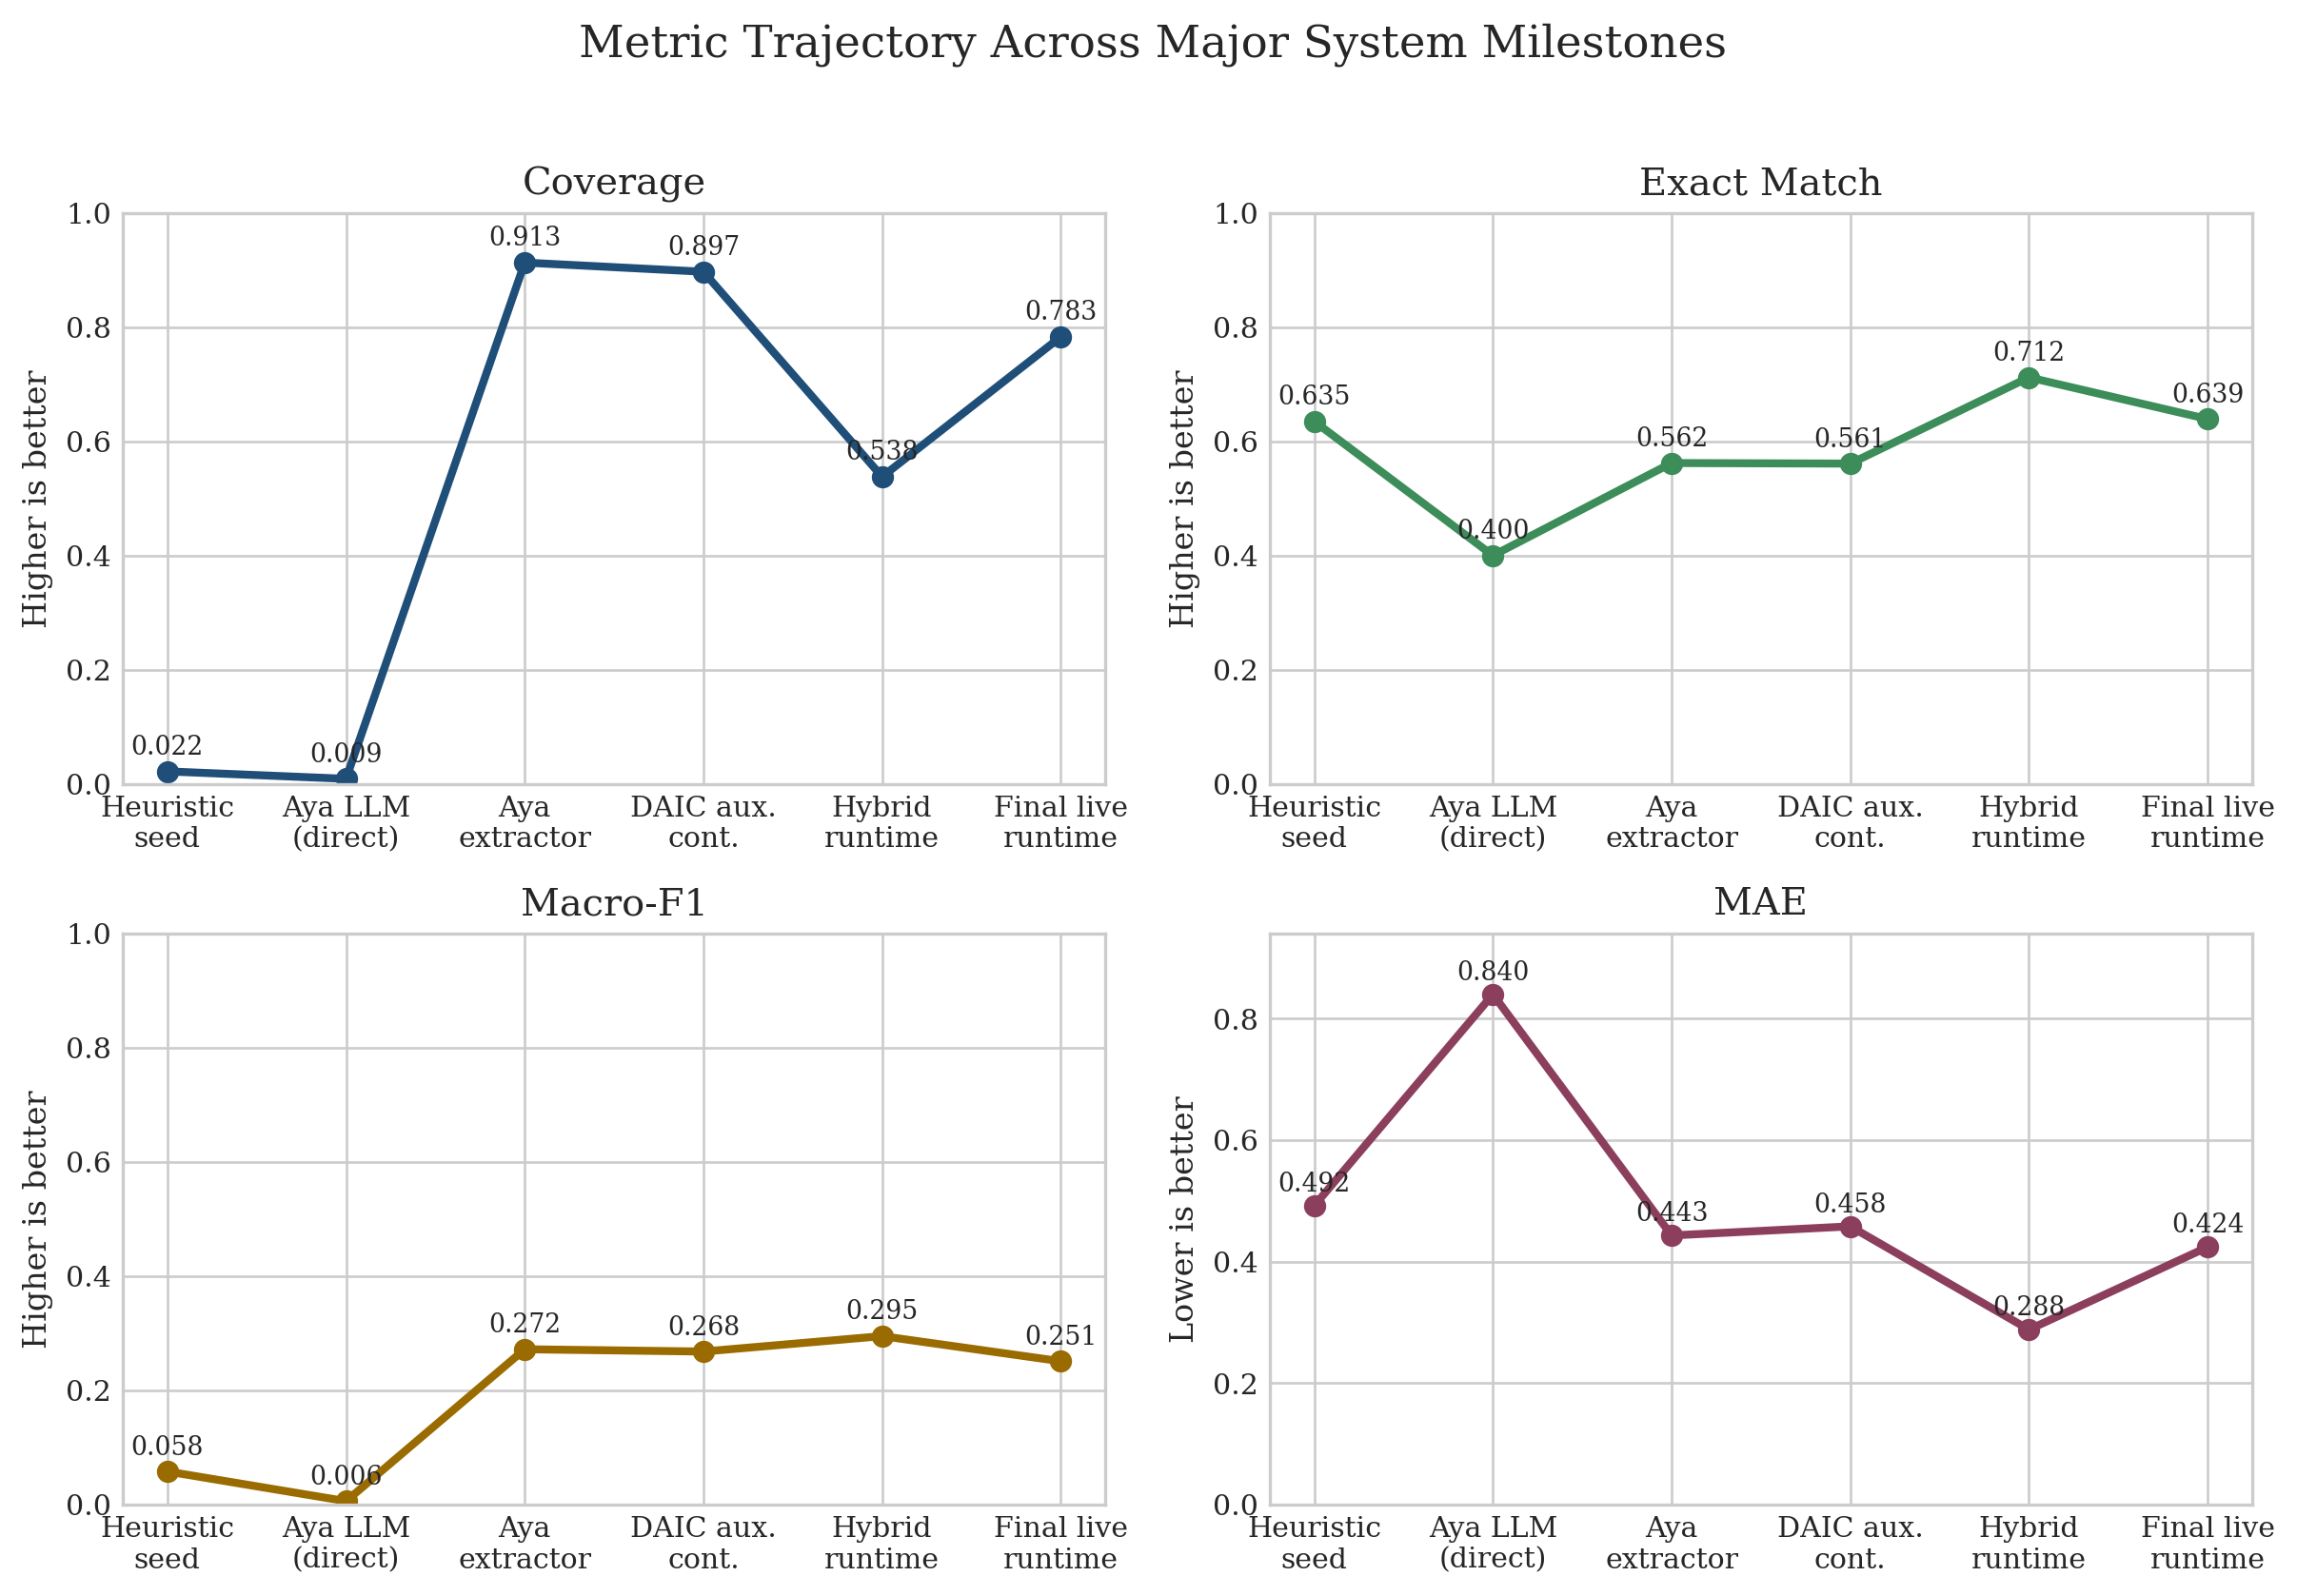
\includegraphics[width=0.88\textwidth]{figures/metric_trajectory.png}
  \caption{Metric trajectory across the major system milestones. The biggest structural jump is from sparse heuristics or raw prompting to the Aya extractor stage, where coverage rises from 0.022/0.009 to 0.913. The later productization phases show a different trade-off: hybrid safety sharply improves end-to-end safety behavior, temporarily depresses coverage, and then recovers much of it through targeted coverage engineering.}
  \label{fig:trajectory}
\end{figure*}

The final runtime combines six components: (1) profile-aware onboarding, (2) a dialogue planner that selects the next best topic/question, (3) an evidence engine, (4) PHQ/GAD item scoring, (5) hybrid safety fusion, and (6) response generation with optional voice I/O. The system is grounded in PHQ-9, GAD-7, and a derived knowledge layer built from questionnaire structure plus NIMH public guidance for generalized anxiety and suicide warning signals \citep{nimh2026gad,nimh2026suicide}. The orchestration logic follows an explicit graph/state style similar to LangGraph-style controllers, which made confidence tracking and escalation easier to inspect \citep{langgraph2026}.

The initial baseline was purely heuristic: topic lexicons, direct cue matching, and hand-written routing. It was enough to bootstrap the UI and the schema, but not enough to behave like a real screener. We also briefly tested raw transcript scoring without the structured extractor path and saw the same pattern: outputs could sound reasonable while touching almost none of the required items. At that point the project moved firmly toward evidence-first extraction. A saved local Qwen2.5-1.5B LoRA checkpoint probe over one English, one Hindi, and one Hinglish held-out example reached 0.429 coverage, 0.667 exact match, and 0.129 macro-F1, but the Hindi case collapsed into a parse failure. That result mattered less for its absolute score than for what it revealed operationally: a compact local model could sometimes follow the schema, but it was still too brittle to anchor multilingual extraction. Aya was the first model family in our pipeline to produce a strong archived multilingual result with stable cross-language evidence behavior \citep{cohere2024aya,kakwani2020indicnlpsuite,nayak2022hingbert}.

We then added a separate safety stack because extractor-only safety was unreliable. A standalone Indic-oriented safety checkpoint reached 0.655 accuracy and 0.473 macro-F1 on the local safety evaluation, which was not sufficient by itself but was good enough to become a useful signal in a fused safety stack. Hybrid fusion initially over-triggered, then later calibration made extractor safety advisory rather than decisive unless corroborated by the runtime safety modules. This was the turning point that pushed the live runtime to 1.0 safety precision and 1.0 safety recall on the held-out runtime endpoint evaluation.

Coverage recovery came later and required language-specific engineering. We first tried a DAIC-WOZ auxiliary continuation run (\texttt{v2run3}) to sharpen English depression-style extraction. That run reached 0.897 coverage and 0.268 macro-F1, but safety recall dropped to 0.312, so we kept DAIC-WOZ as an auxiliary English-only option rather than the main path. A later full rerun of the Aya continuation setup (48-example held-out evaluation) reached 0.943 coverage, 0.614 exact match, 0.297 macro-F1, and 1.0/1.0 safety precision/recall with zero parse failures. The stronger solution for deployment remained architectural: coverage-aware planning, expanded Hindi lexicons, better negation handling, English windowed extraction, and a verifier path for ambiguous anxiety items. The final deployment later moved to self-hosted local inference with a smaller Qwen2.5 Instruct runtime \citep{qwen2026qwen25}, while cloud speech-to-text/text-to-speech handled voice I/O \citep{google2026stt,google2026tts,google2026cloudrun}.

\paragraph{What was actually used in the project.}
Because the project evolved over many milestones, it is important to separate systems that shaped the final build from models that only appeared in planning notes. The main measured project path is: heuristic screening, a saved local Qwen2.5-1.5B probe, Aya extraction, Aya continuation with DAIC-WOZ auxiliary supervision, the standalone Indic safety checkpoint, hybrid runtime validation, and the final self-hosted local runtime. The DAIC continuation run \texttt{v2run3} was logged and used for decisions, but was not stored as a standalone repo JSON report. We also ran a later retrospective local Llama 3.1 8B quantized probe on the same three-example multilingual slice used for the saved Qwen probe. That comparison is useful for model-selection hindsight, but it is not presented as a historical milestone because it was run after the main Aya decision had already been made. Mistral NeMo 12B and Gemma 3 12B appear in planning documents, but we did not find final archived held-out result files for them in the repo \citep{mistral2026nemo,google2026gemma}.

\begin{table*}[t]
\centering
\small
\setlength{\tabcolsep}{4.5pt}
\begin{tabular}{lccccc}
\toprule
System milestone & Coverage & Exact & Macro-F1 & Safety P/R & Main inference \\
\midrule
Heuristic seed runtime & 0.022 & 0.635 & 0.058 & 1.000 / 0.604 & rules + lexicons \\
Early raw Aya scoring check & 0.009 & 0.400 & 0.006 & 0.667 / 0.038 & hosted Aya prompt \\
Local Qwen2.5-1.5B probe (\textit{n}=3) & 0.429 & 0.667 & 0.129 & 0.000 / 0.000 & saved LoRA checkpoint \\
Retrospective Llama 3.1 8B probe (\textit{n}=3) & 0.893 & 0.640 & 0.190 & 0.000 / 0.000 & local MLX 4-bit probe \\
Aya extractor offline baseline & 0.913 & 0.562 & 0.272 & 0.000 / 0.000 & hosted Aya extractor \\
DAIC auxiliary continuation (\texttt{v2run3}) & 0.897 & 0.561 & 0.268 & 1.000 / 0.312 & Aya continuation log \\
Aya continuation full rerun (local-base VM) & 0.943 & 0.614 & 0.297 & 1.000 / 1.000 & Aya local-base + adapter \\
Hybrid runtime validation & 0.538 & 0.712 & 0.295 & 1.000 / 1.000 & fused runtime + safety \\
\textbf{Final live runtime} & \textbf{0.783} & \textbf{0.639} & \textbf{0.251} & \textbf{1.000 / 1.000} & \textbf{self-hosted local runtime} \\
\bottomrule
\end{tabular}
  \caption{End-to-end milestone comparison restricted to systems for which we have either archived reports, saved probe artifacts, or explicit logged continuation summaries. The counter-intuitive result is that the best offline extractor is not the best deployed system. The extractor wins on raw coverage, but it completely fails safety. The saved local Qwen probe documents an early compact-model experiment, while the retrospective local Llama probe provides a later open-model check. Neither displaced Aya as the extractor backbone because Aya remained the first strong archived multilingual result. The DAIC continuation row comes from a Colab experiment log captured during the project run, while the continuation full-rerun row is from an archived full held-out summary JSON.}
\label{tab:milestones}
\end{table*}

\section{Results and Observations}
Table~\ref{tab:milestones} and Figure~\ref{fig:trajectory} show the project's most important empirical caution: \emph{exact match alone was misleading early on}. The heuristic baseline reported 0.635 exact match, but only 0.022 coverage. In practice this meant the system was abstaining on most items, so the exact-match number reflected sparsity more than clinical usefulness. The same logic explains why the early raw Aya scoring check was unusable: it was fluent, but clinically almost silent. The saved local Qwen probe sharpened that point further. It produced structured output on English and Hinglish, but failed outright on the Hindi case. The lesson was not that Qwen was ``bad'' in general; it was that a narrow schema-following success was not enough to justify multilingual extractor selection.

The large offline Aya extractor was the first system that behaved like a real screening engine. It pushed coverage to 0.913 with 0 parse failures and fairly balanced multilingual behavior (0.922 English, 0.852 Hindi, 0.973 Hinglish coverage). Just as importantly, its strength was broad rather than accidental: it performed well on all three language conditions instead of only on the easiest English slice. But that success surfaced the next problem. High extractor coverage did not imply safe deployment. In the held-out extractor evaluation, safety precision and recall were both zero, so the system could fill in questionnaire items while still being unsafe as an autonomous front-end.

The hybrid runtime reversed this trade-off. Early hybrid validation hit 1.0 precision and recall for safety, but coverage collapsed to 0.538. That dip matters because it shows that safety fusion, routing, and runtime conservatism were not free. The later coverage-focused passes were therefore targeted rather than broad: expanded Hindi lexicons, improved negation handling, windowed English extraction, and verifier logic for English worry/relaxation items. The final live system recovers to 0.783 coverage, 0.639 exact match, and 0.251 macro-F1 while keeping 1.0/1.0 safety and zero parse failures. Compared with the best offline Aya extractor, the live system still trails by 0.130 coverage and 0.021 macro-F1, but gains 1.0 absolute safety precision and 1.0 absolute safety recall. For a deployed screening partner, that was the more defensible operating point.

\paragraph{Retrospective open-model comparison.}
After the main pipeline had stabilized, we ran a local quantized Llama 3.1 8B probe on the same three-example multilingual slice used for the saved Qwen probe. The result reached 0.893 coverage, 0.640 exact match, and 0.190 macro-F1, which is notably stronger than the saved Qwen probe on raw coverage but still weaker than the archived Aya extractor on the main held-out metric. More importantly, the probe over-escalated safety on benign examples (\texttt{review} for English and \texttt{urgent} for Hinglish), so it did not undermine the earlier choice of Aya as the extractor backbone. In other words, the retrospective Llama run was useful as a check on model-selection hindsight, but it did not change the conclusion drawn from the archived multilingual evaluation.

\begin{figure*}[t]
  \centering
  \begin{subfigure}[t]{0.64\textwidth}
    \centering
    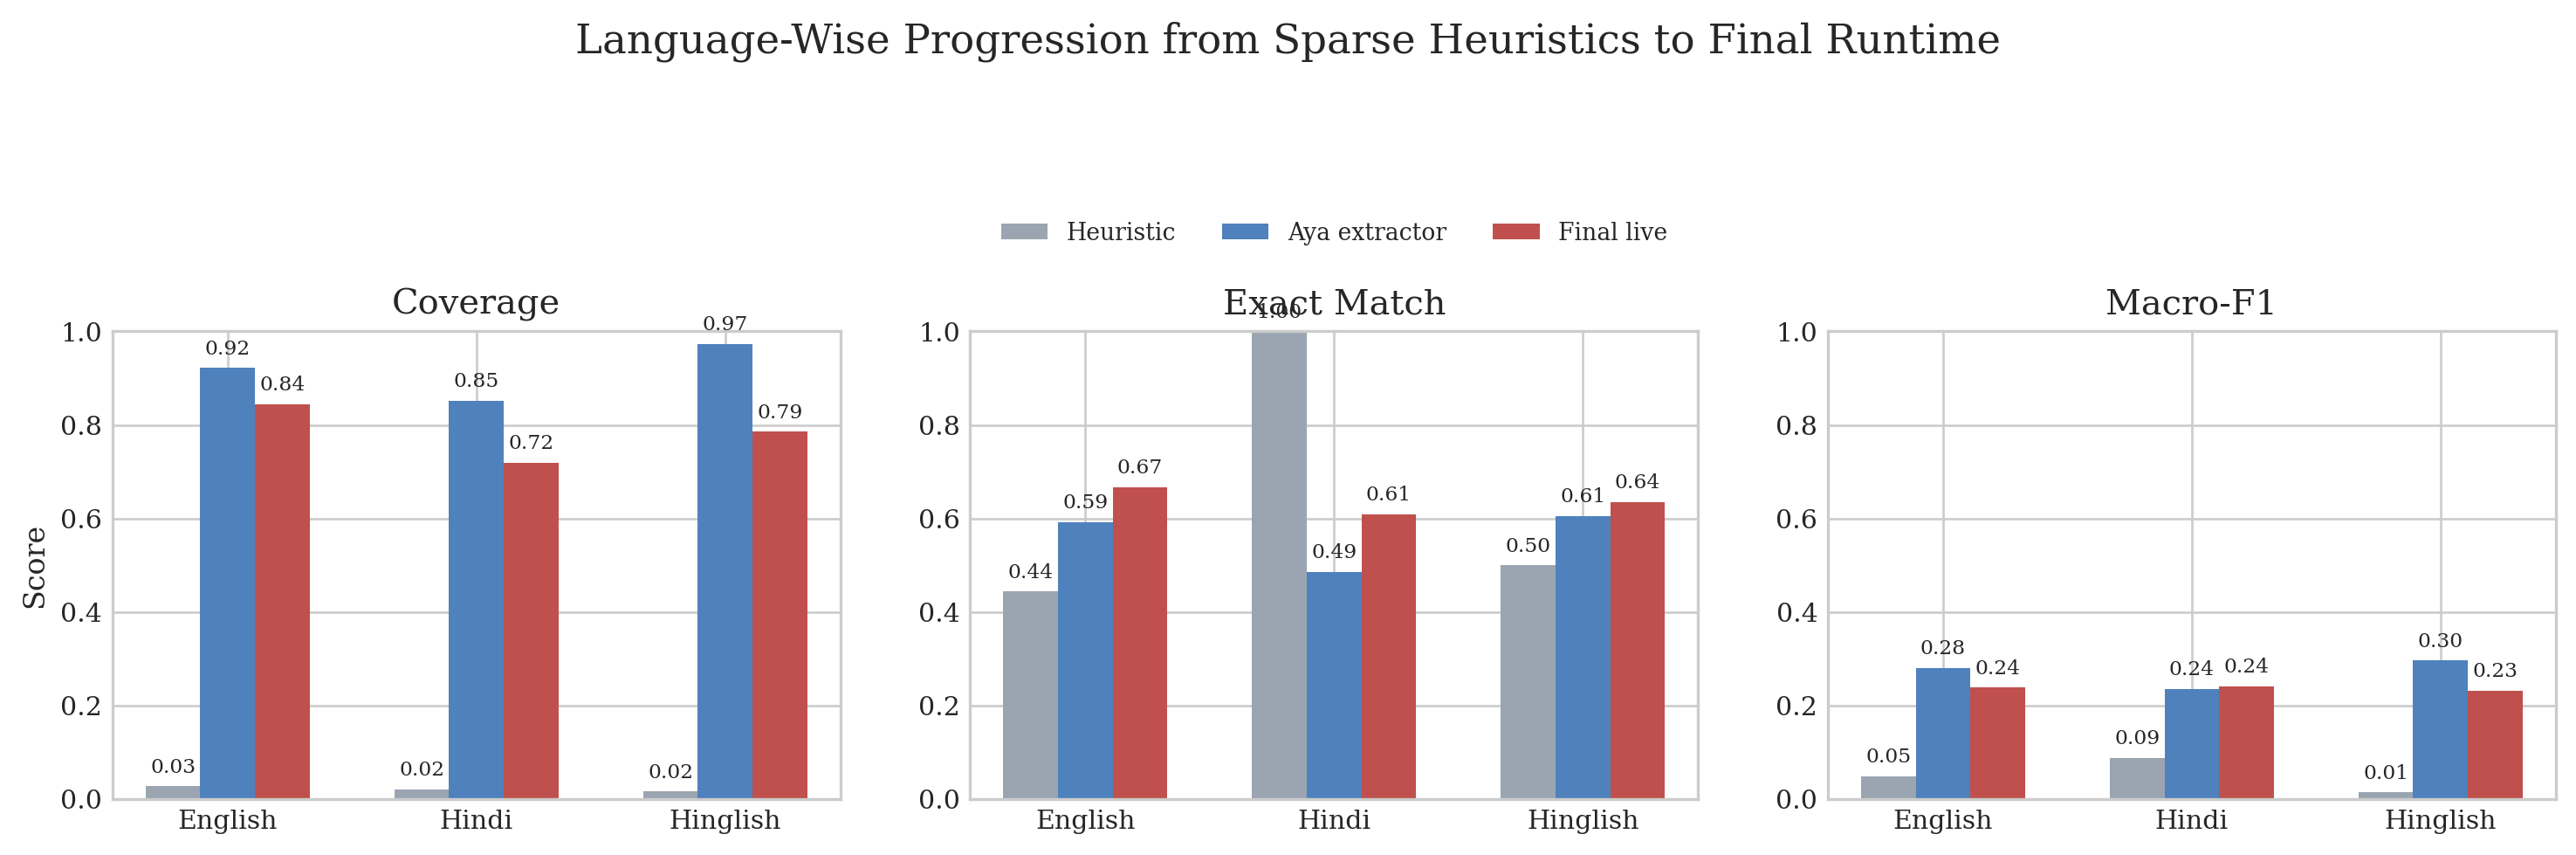
\includegraphics[width=\textwidth]{figures/language_comparison.png}
    \caption{Language-wise progression}
  \end{subfigure}
  \hfill
  \begin{subfigure}[t]{0.34\textwidth}
    \centering
    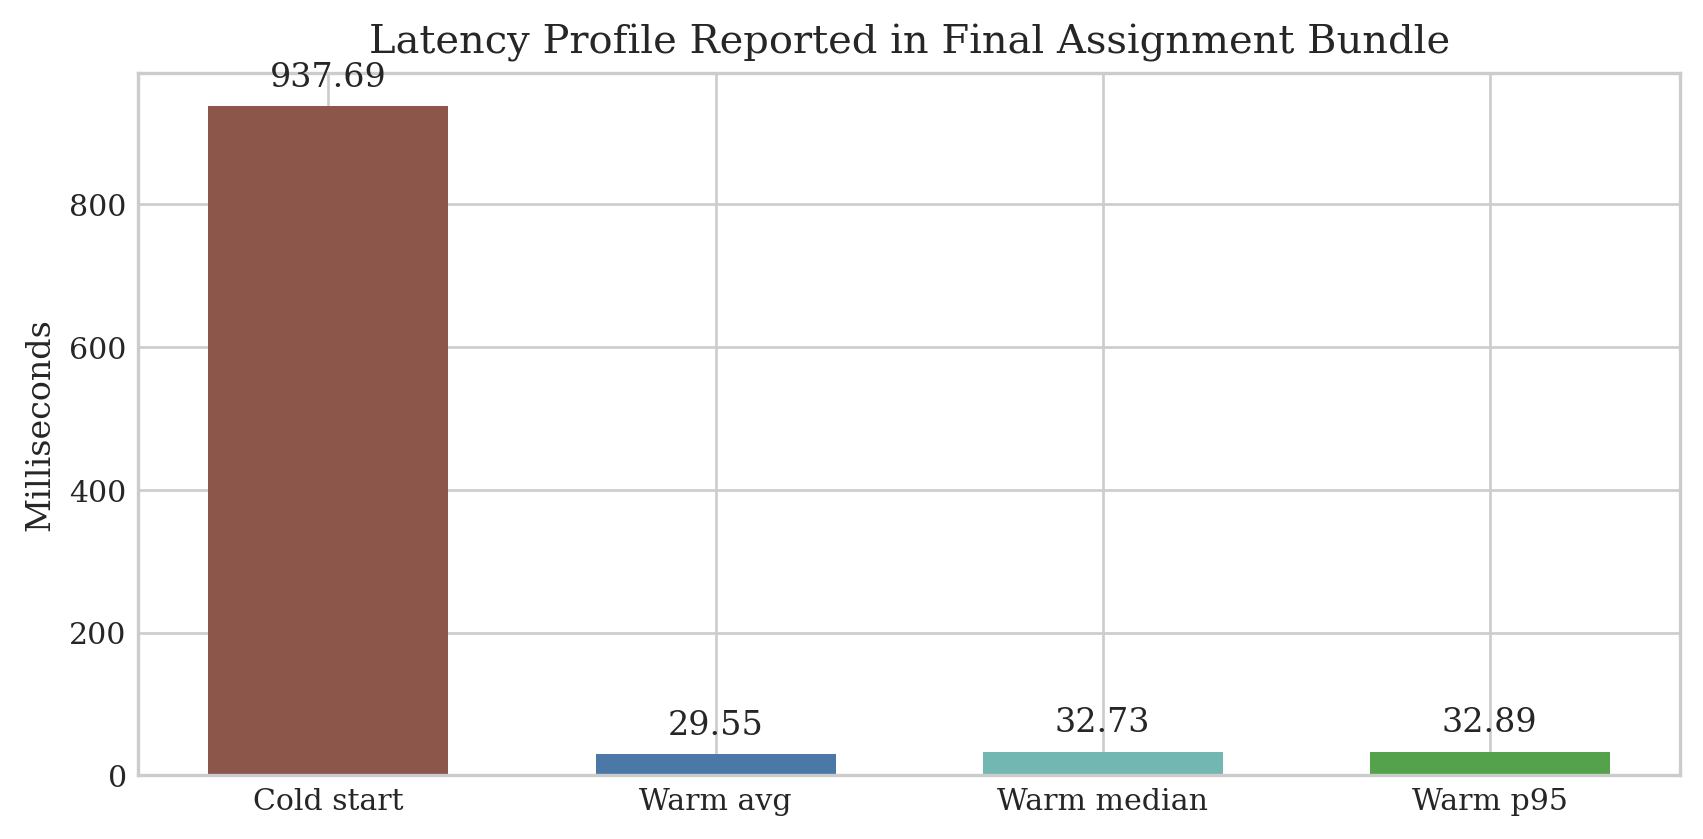
\includegraphics[width=\textwidth]{figures/latency_profile.png}
    \caption{Final latency profile}
  \end{subfigure}
  \caption{Language-wise progress and deployment latency. The left panel shows that the final runtime does not simply inherit the extractor's language profile: English becomes the strongest slice only after windowed extraction and a verifier are added, while Hindi remains the weakest final slice. The right panel shows that the deterministic screening path is fast once warm, but this should not be over-interpreted as a full spoken-dialogue round-trip measure.}
  \label{fig:lang-latency}
\end{figure*}

Figure~\ref{fig:lang-latency} reveals the most important language pattern. The extractor-only stage was already strong in Hinglish and English, but the final live runtime becomes strongest in English (0.844 coverage) only after the late English-specific repair cycle. That cycle added windowed extraction, an English verifier pass, and targeted disambiguation for \texttt{gad\_q2}, \texttt{gad\_q3}, and \texttt{gad\_q4}; all three of those items eventually reached full coverage and exact match in English. Hindi, by contrast, becomes the weakest final slice at 0.719 coverage. This is not because the system ignores Hindi entirely, but because it still misses a few sparse symptom types more often than English and Hinglish. The heatmap in Figure~\ref{fig:heatmap} makes this visible at the item level.

\begin{figure*}[t]
  \centering
  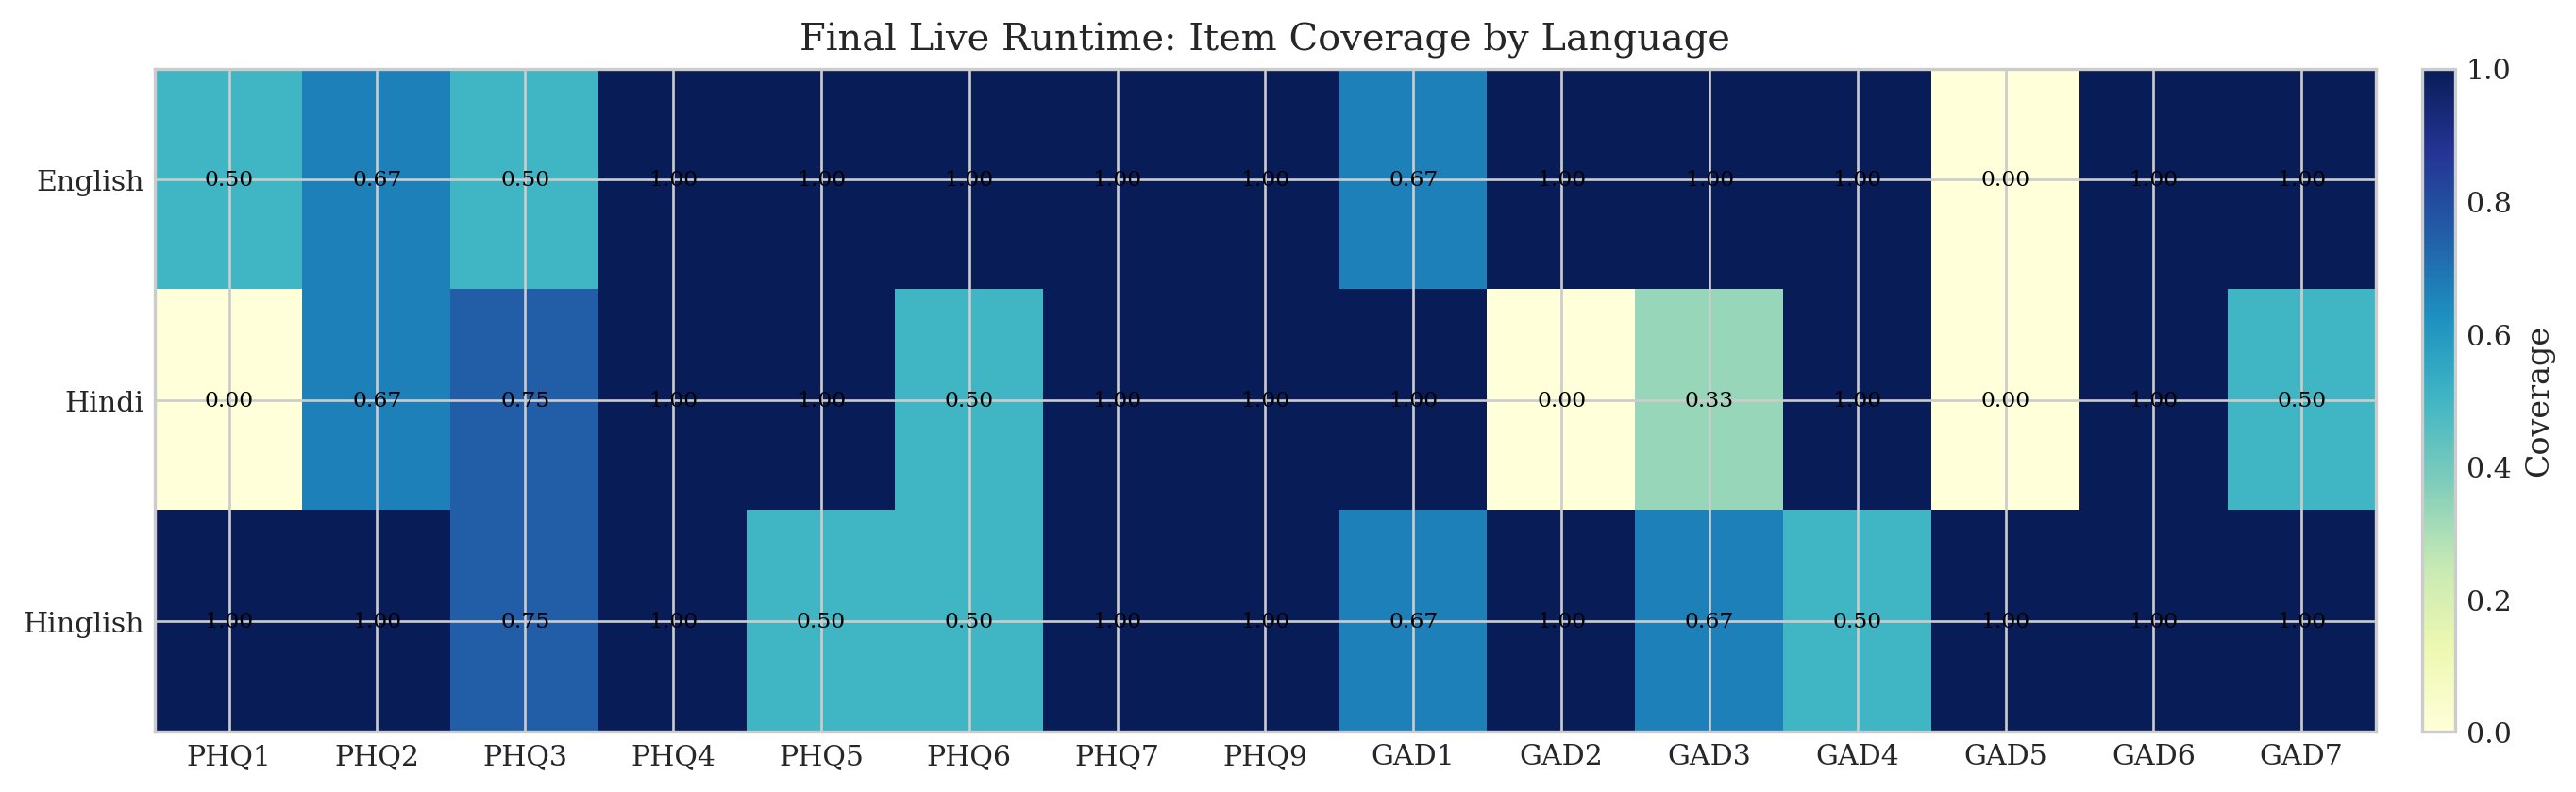
\includegraphics[width=0.88\textwidth]{figures/item_coverage_heatmap.png}
  \caption{Final live runtime item coverage by language. The most useful inference is not that the system is uniformly strong, but that its remaining misses are concentrated. Hindi still drops \texttt{PHQ1} and \texttt{GAD2} to zero coverage and under-covers \texttt{GAD3}, while Hinglish remains broad but less exact on a few somatic items. English coverage is no longer the bottleneck; its remaining errors are mostly calibration rather than missing evidence.}
  \label{fig:heatmap}
\end{figure*}

The final multilingual breakdown is balanced enough for the project goal, but still diagnostic of where the system needs work next. English reaches 0.844 coverage, 0.667 exact match, and 0.239 macro-F1. Hindi reaches 0.719 / 0.609 / 0.242. Hinglish reaches 0.786 / 0.636 / 0.232. The most important observation here is that coverage and macro-F1 do not move identically. Hinglish stays competitive on coverage, but exactness on items such as appetite and sleep still lags because code-mixed cues can be recognized without being perfectly severity-calibrated. The Hindi row in Figure~\ref{fig:heatmap} shows a different problem: missing evidence rather than merely mis-scored evidence.

The safety story is also worth separating into two layers. The standalone local safety checkpoint is only moderately strong on its own (0.607 accuracy, 0.437 macro-F1 in archived local evaluation), but once fused with rules and runtime corroboration it becomes very effective end-to-end. This is an important project result because it shows why a single monolithic conversational model is the wrong abstraction for risk-sensitive screening. The hybrid stack performed better than any individual component on the actual screening objective.

\section{Deployment, Voice, and Limitations}
By the final milestone, ManoVarta was not just an offline evaluation artifact. The system exposed patient-profile onboarding, a reviewer path, live voice endpoints, a public runtime, and self-hosted inference. The final deployment config reports \texttt{provider=local}, self-hosted inference enabled, hybrid safety enabled, and local safety checkpoint enabled. The deployed self-hosted stack uses local Qwen2.5 runtime weights for chat and extraction rather than hosted Hugging Face inference. Browser voice remains available, but the final voice path also includes backend Google Cloud speech-to-text and text-to-speech, which makes the system meaningfully more robust than a browser-only microphone wrapper \citep{google2026stt,google2026tts}. The assignment bundle reports 2.292 average user turns to a stable item score and warm-path latency around 8 ms (8.18 ms average, 8.0 ms median, 8.7 ms p95).

At the same time, several limitations remain. First, even with a complete 60-session gold pack, the corpus is still modest and source-heterogeneous; results should be treated as system validation rather than clinical validation. Second, DAIC-WOZ is useful as auxiliary English supervision, but the project's own experiments confirmed the caution from \citet{burdisso2024daic}: it is a poor substitute for genuine multilingual item labels. Third, we intentionally do not claim final Mistral NeMo or Gemma results because the repo contains planning references for both, but no completed, reproducible held-out result files. Fourth, both the local Qwen2.5 and retrospective Llama 3.1 results reported here are probe artifacts rather than full multilingual held-out benchmarks. Fifth, our latest numbers now include both the shipped runtime and a full Aya continuation rerun; a dedicated long-cycle retrain/fine-tune pass over the finalized 60-session human-adjudicated set is still staged as the next training experiment. Finally, even perfect held-out safety precision/recall in this project should not be interpreted as a guarantee of safe real-world deployment. Human oversight remains mandatory.

\section{Conclusion}
ManoVarta began as an idea to make screening feel less like a form. The project only started to work once we stopped treating conversational fluency as enough and instead enforced structure: evidence before scoring, safety outside the main generator, language-aware repair loops, and explicit deployment validation. The final live system is therefore not the numerically strongest extractor we built, but it is the strongest \emph{screening product} we built: multilingual, voice-capable, self-hosted, zero-parse-failure, and safety-consistent.

The clearest empirical lesson is that productization changed the optimization target. The best offline Aya extractor maximized coverage, but the final live runtime achieved the more balanced outcome: 0.783 coverage, 0.639 exact match, 0.251 macro-F1, 1.0 safety precision, 1.0 safety recall, and rapid stabilization over only 2.29 user turns on average. For future work, the next high-value directions are larger real multilingual data, stronger Hindi item coverage, and tighter end-to-end voice latency. Within the scope of this project, however, ManoVarta successfully demonstrates that conversational multilingual screening can be made both technically grounded and deployment-aware.

\bibliographystyle{acl_natbib}
\bibliography{project2_acl_report}

\end{document}
